\section{Durchführung}
\subsection{Kalibrierung des Magnetfeldes}
Während des Versuchs wird die Magnetfeldstärke nicht gemessen, sondern über den Spulenstrom eingestellt.
Es muss also zunächst die Abhängigkeit von Magnetfeldstärke zu Spulenstrom gemessen werden.
Dafür wird in einem Bereich von \SI{0}{\ampere} bis \SI{22}{\ampere} in Abständen von \SI{1}{\ampere} die Magnetfeldstärke mit einer Hallsonde bestimmt.

\subsection{Messung der roten Spetrallinie}

Die Übergänge, die zur Entstehung der roten Spektrallinie von Cadmium führen, entsprechen dem Übergang von $^1D_2$ zu $^1P_1$.
Ein Termschema für die möglichen Übergänge ist in Abbildung \ref{fig:Term_rot}.
Für diese beiden Zustände gilt $S=0$ und damit $g_J = 1$, es handelt sich hierbei also um den normalen Zeeman-Effekt.
Das Magnetfeld wird nach Gleichung \eqref{eqn:B} auf eine Stärke von \SI{650}{\milli\tesla} eingestellt.
Sowohl die $\pi$- (\SI{0}{\degree}) also auch die $\sigma$-Linie (\SI{90}{\degree}) werden durch den Polarisationsfilter ausgewählt.
Durch den verschiebbaren Spalt des Versuchsaufbaus kann die rote Spetrallinie ausgewählt werden, die Digitalkamera wird so positioniert, dass ein deutliches Interferenzmuster aufgenommen werden kann.

\begin{figure}[H]
  \centering
  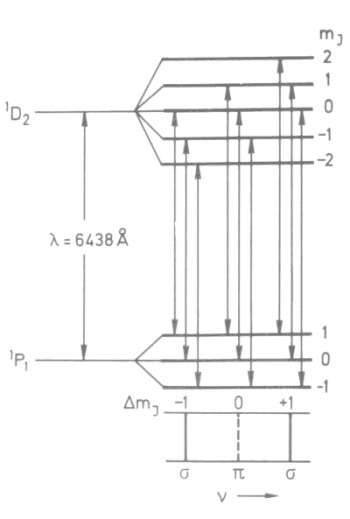
\includegraphics[width = .4\textwidth]{images/Termschema_rot_TUbes.jpg}
  \caption{Termschema für die Übergänge der roten Spektrallinie. Die Übergänge sind nach den Auswahlregeln geordnet aufgetragen. Jeder dieser Übergaänge hat den Landé-Faktor $g=1$ \cite{WWW}.}
  \label{fig:Term_rot}
\end{figure}

\subsection{Messung der blauen Spektrallinie}
Der Übergang von $^3P_1$ zu $^3S_1$ erzeugt die blaue Spektrallinie von Cadmium.
Für beide Niveaus gilt $S=1$, somit folgt für die Landé-Faktoren $g_J(^3P_1) = \num{1.5}$ und $g_J(^3S_1) = \num{2}$.
Nach Gleichung \ref{eqn:an_zeeman} kann dann für die möglichen Übergange die Energie $\Delta E$ bestimmt werden.
Für Übergange mit $\Delta m = \pm 1$ unterscheiden sich die Energien für die unterschiedliche $m_1$ und $m_2$, weswegen der Landé-Faktor zu $|g_J| = \num{1.75}$ für die $\sigma$-Linie berechnet wird.
Für Übergange mit $\Delta m = 0$ beträgt der Landé-Faktor für alle möglichen Übergange $|g_J| = \num{0.5}$.
Dieser wird auch für die Einstellung des Magnetfeldes zur Messung der $\pi$-Linie genutzt.
Das Termschema für die Übergänge der blauen Spektrallinie sind in Abbildung \ref{fig:Term_blau} dargestellt.
Die zwei Magnetfelder der Stärke \SI{280}{\milli\tesla} für die $\pi$-Linie und \SI{1120}{\milli\tesla} für die $\sigma$-Linie werden daraufhin festgelegt.
Auch hier wird der Polarisationsfilter für die beiden Linien eingestellt.
\\
\begin{figure}[H]
  \centering
  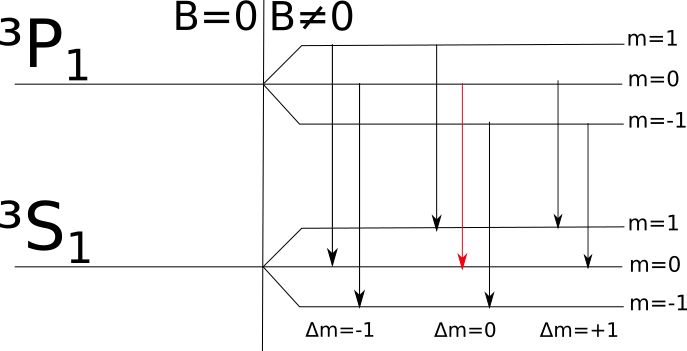
\includegraphics[width = .6\textwidth]{images/Term_blau.png}
  \caption{Termschema für die Übergänge der blauen Spektrallinie. Die Übergänge sind nach den Auswahlregeln geordnet aufgetragen. Jeder dieser Übergaänge hat den Landé-Faktor $g=1$. Der \textcolor{red}{rote} Übergang von $m_1 = 0$ zu $m_2=0$ ist zwar nach den Auswahlregeln erlaubt, aber sehr unwahrscheinlich.}
  \label{fig:Term_blau}
\end{figure}
